\documentclass{article}

\textwidth=6.5in
\textheight=8.5in
\voffset=-54pt
\oddsidemargin=0in
\evensidemargin=0in
\setlength{\parskip}{8pt}
\setlength{\parindent}{0pt}

\usepackage{workbook}

\usepackage{handout}

\usepackage{exam}

\newcommand{\answerbox}[3][]{
    \fbox{\begin{minipage}[t][#2][c]{#3}
        Final answer: #1
    \end{minipage}}
    }

\begin{document}

 

 \noindent
{\large \mbox{} \hfill \bf Name:\underline{\hspace{2.8in}}}

 {\mbox{} \hfill \it (Please write your name neatly in print.)}


 
\medskip
 
\noindent
{\large\bf
Integration Skills Check \\ Math Mb Spring 2025}
\noindent






\iffalse
\begin{center}
\begin{tabular}{|c|c|c|}
\hline
Problem & Points & Score\\ \hline
& &\\
1 &  & \\ 
\hline
&& \\
2&  &  \\ 
\hline
& &\\
3&&  \\ 
 \hline
& &\\
Total&  &  \\ 
& &\\ \hline

\end{tabular}
\end{center}
\fi


{\Large
\begin{center}\textbf{Directions---Please read carefully!} \end{center}}

You have 60 minutes to complete this Skills Check. \textbf{Calculators or any other aids are not permitted.}  


For each problem, write your final answer in the answer box provided. You may do work on any page and may ask for scratch paper, but \textbf{no work or writing outside of the answer box will be graded.}

Write neatly, as answers that cannot be read will not receive credit. 

   

\begin{center}\textbf{Good luck!}\end{center}



\newpage

\begin{enumerate}

\item Find the following basic \textbf{indefinite} integrals.

\begin{enumerate}
    \item $\displaystyle \int x^n \;dx$ (for $n \neq -1$)

    \vfill 

    \answerbox{.5 in}{5.5 in}
    
    \item $\displaystyle \int \sin(x) \;dx$

    \vfill 

    \answerbox{.5 in}{5.5 in}
    \item $\displaystyle \int e^x \;dx$

    \vfill 
    \answerbox{.5 in}{5.5 in}

    \item $\displaystyle \int \frac{1}{1+x^2} \;dx$

    \vfill 

    \answerbox{.5 in}{5.5 in}
    \item $\displaystyle \int \frac{1}{x}\;dx $
    
    \vfill 

    \answerbox{.5 in}{5.5 in}
    \item $\displaystyle \int \cos(x)\;dx$

    \vfill 

    \answerbox{.5 in}{5.5 in}

\end{enumerate}

\newpage 



\item Find each integral. You may use any method. \textbf{Fully simplify your answers for all definite integrals.}
\begin{enumerate}

    \item $\displaystyle \int \big(7x^5 -  3x^4\big) \, dx$

        \vfill 

        \answerbox{.5 in}{5.5 in}
    
    \item $\displaystyle \int_{-424}^{424} x^{2025}\,dx$ 

        \vfill 

        \answerbox{.5 in}{5.5 in}
    \item $ \displaystyle \int_{-5}^{5} \sqrt{25-x^2} \,dx$

         \vfill 

         \answerbox{.5 in}{5.5 in}

    \newpage 
    
    \item $\displaystyle \int (x-1)\sqrt{x} \,dx$

        \vfill 

        \answerbox{.5 in}{5.5 in}

        \item $\displaystyle \int x\sqrt{x-1}\,dx$

    \vfill 

       \answerbox{.5 in}{5.5 in}

    \newpage
    
    \item $ \displaystyle \int_{0}^{\sqrt{\pi}} x\sin(x^2)\, dx$

        \vfill 

        \answerbox{.5 in}{5.5 in}
    \item $\displaystyle \int x^2\sin (3x) \,dx$

        \vfill 

        \answerbox{.5 in}{5.5 in}

    \newpage 
    \item $\displaystyle \int_1^e x\ln x \,dx$

        \vfill 

        \answerbox{.5 in}{5.5 in}
    \item $\displaystyle \int \tan x\,dx$

        \vfill 

        \answerbox{.5 in}{5.5 in}




\end{enumerate}

\newpage 

\item We want to approximate the area of the region $\mathcal{R}$ shown below using a right Riemann sum with 15 equal sub-intervals, $R_{15}$. $\mathcal{R}$ is bounded by the curves $y=f(x)$, $y=0$, $x=4$, and $x=9$, where $f(x)=\sqrt x$.

    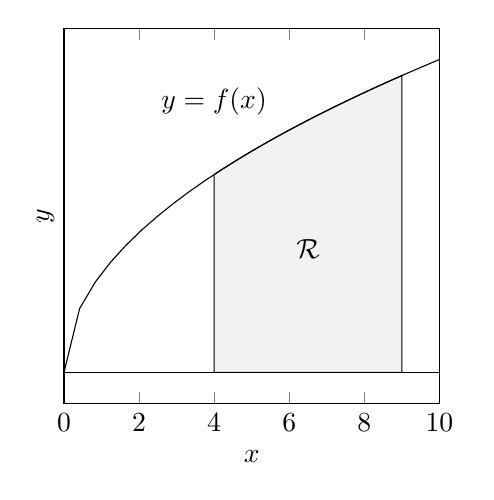
\begin{tikzpicture} 
      \begin{axis}[ cycle list={black}, xmin=0, xmax=10, 
        width=2.5in, height=2.5in, clip=false, ytick=\empty, 
        xlabel=$x$, ylabel=$y$] 
        \addplot+[domain=0:10]{0} node [right] {\;} ; 
        \addplot+[domain=4:9, fill=lightgray, fill opacity=0.2] 
        {sqrt(x)} \closedcycle; 
        \addplot+[domain=0:10] {sqrt(x)}; 
        \node [above] at (axis cs: 4, 2.5) {$y=f(x)$};
        \node at (axis cs: 6.5, 1.25) {$\mathcal{R}$};
      \end{axis} 
    \end{tikzpicture}
\begin{enumerate}

    \item Write down the value of $\Delta x$.
    \vfill

    \answerbox[$\Delta x =$]{.5 in}{5.5 in}
    
    \item Write down a formula for $x_k$, the right endpoint of the $k$th sub-interval.
    \vfill
    
    \answerbox[$x_k=$]{.5 in}{5.5 in}
    
    \item Write down a formula for $R_{15}$ using sigma notation. 
    \vfill
    
    \answerbox[$R_{15}=$]{.75 in}{5.5 in}
\end{enumerate}
    
    
\end{enumerate}




\end{document}